
\section{Simulation results}
I have implemented a simulated surface vessel and a non-buoyant subsurface vessel, both of which are controllable either manually or by automated controller. The two vessels are bound together by a wire tether. The vessels and the wire are all affected by weather effects such as ocean currents, as well as physical effects like added mass and inertia. 

The simulation works as would be intuitively expected. An example of the simulation graphical interface can be seen in \cref{fig:sim-display}. The figure shows a surface vessel and the ROV under water in green, and the teal tether connecting them. The simulated water is shown as a grey volume, but it's not easy to distinguish it in \cref{fig:sim-display} because it takes up the entire screen. 

\begin{figure}
	\centering
	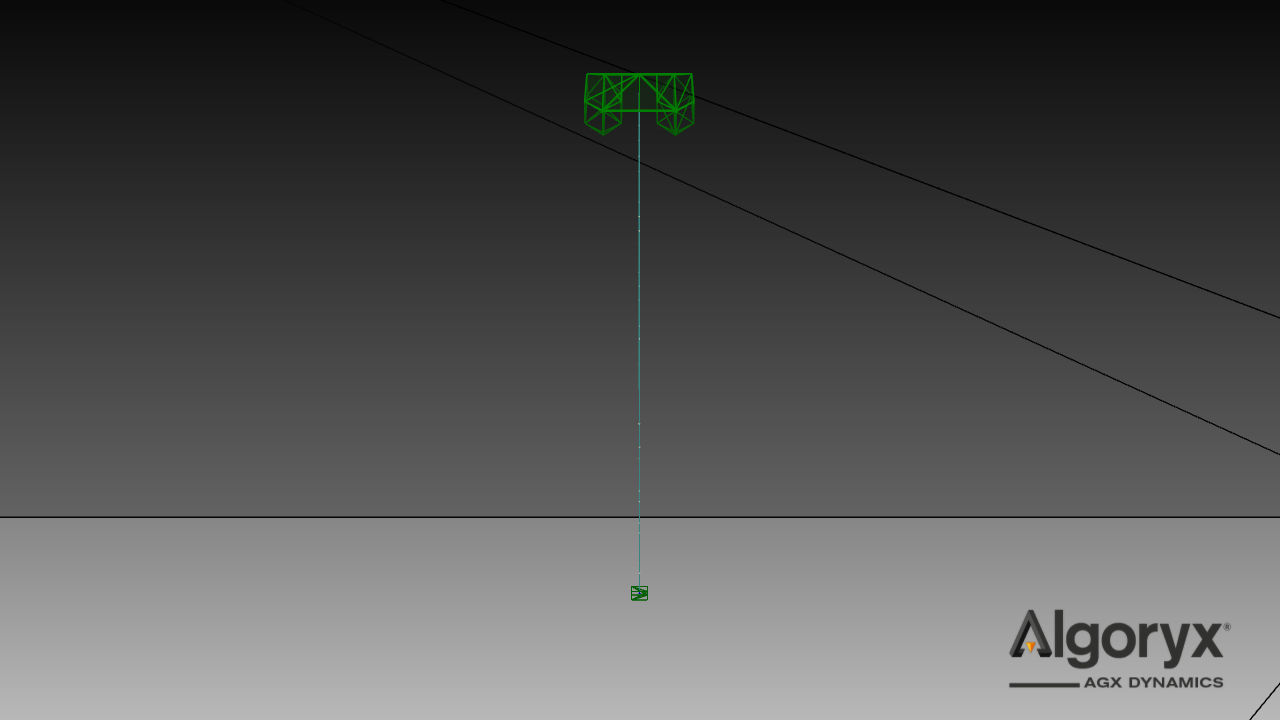
\includegraphics[width=0.7\textwidth]{sim-display}
	\caption{The graphical user interface of AGX with the simulation running}
	\label{fig:sim-display}
\end{figure}


\section{Control system results}
